\chapter{Expample chapter žščřcjďťň}
\label{chap:Expample}

\lipsum[1]

\begin{lstlisting}
for i = 1:50
	disp(i)			% comment         
end
\end{lstlisting}

\begin{figure}[!h] 
	\begin{center}
		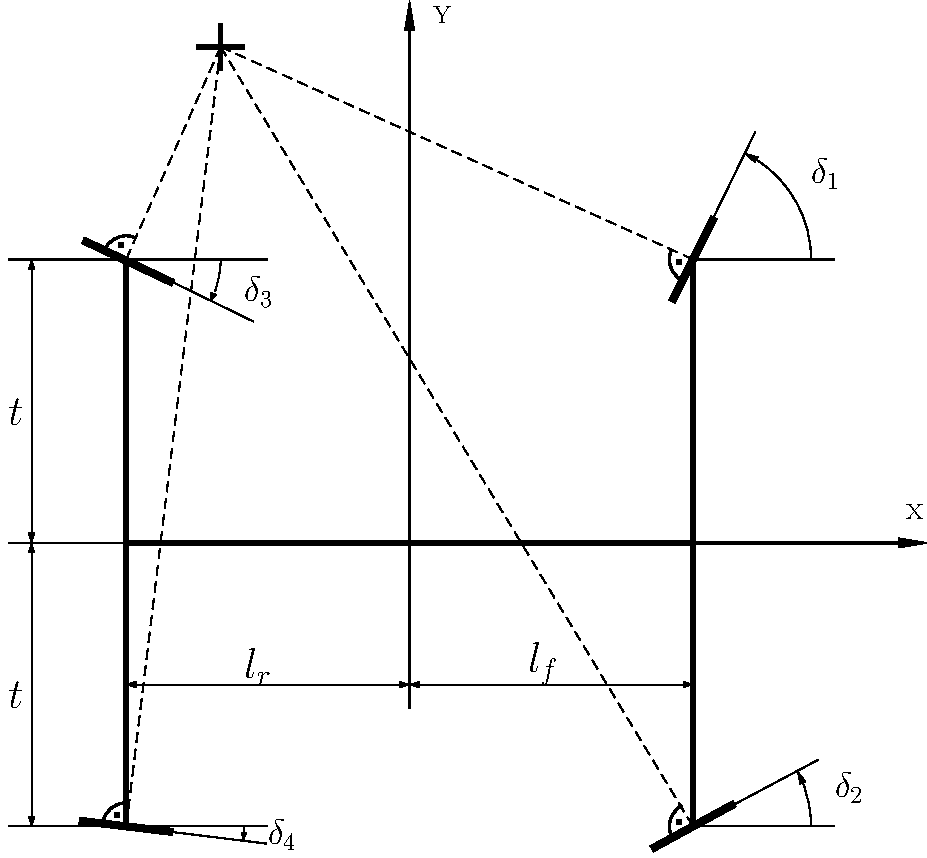
\includegraphics[scale=0.4]{images/example_fig.pdf}
	\end{center}
	\caption[Caption in list of figures]{Caption of the figure}
	\label{fig:figurelabel}
\end{figure}	

\lipsum[2]

\begin{equation}\label{eq:DCmot}
U(t) = Ri(t) + L\cdot\frac{di(t)}{dt} + C\omega(t)
\end{equation}

Pokud máme model popsaný rovnicí \ref{eq:LS_model}, kde \boldmath $\hat{y}$ je odhad výstupu modelu, $b = \left[b_1,b_2,...,b_n\right]^T$ jsou parametry modelu a $X = \left[x_1,x_2,...,x_n\right]$ jsou vstupy modelu, \unboldmath

\begin{center}
	\begin{tabular}{|l|l|}
%		\hline 
		&  \\ 
		\hline 
		a & 787 \\ 
%		\hline 
		b & 788 \\ 
%		\hline 
		d & 77575 \\ 
%		\hline 
		gf & 7 \\ 
%		\hline 
		h & 6 \\ 
%		\hline 
		hrf & 7 \\ 
%		\hline 
	\end{tabular} 
\end{center}


\begin{equation}\label{eq:LS_model}
\hat{y} = \bm{X} \bm{b}
\end{equation}

\section{Example section}
\label{sec:Example-section}

\begin{equation}\label{eq:DCmot2}
U(t) = Ri(t) + L\cdot\frac{di(t)}{dt} + C\omega(t)
\end{equation}


V kapitole \ref{chap:Expample} \textbf{\textit{v sekci}} \ref{sec:Example-subsection} v obrazku \ref{fig:figurelabel} podle rovnice \ref{eq:DCmot} jak je uvedeno v \cite{Blaha}.




\subsection{Example subsection}
\label{sec:Example-subsection}
\lipsum[6]
\lipsum[7]


\begin{table}[!h] % tabulka parametrů Car4
	\begin{center}
		\begin{tabular}{ccc}
			a	& b & c \\ 
			ab	& cd & ef \\ 
			a	& b &  c\\ 
			a	& b &  c

		\end{tabular}
	\end{center}
	\caption[Kratky popisek tabulky]{Popisek Tabulky \cite{Atkeson1996}}
	\label{tab:car4Param}
\end{table}


\lipsum

\begin{figure}[!ht] 
	\begin{center}
		%		\includegraphics[width=\textwidth]{images/LLM_init.pdf}
	\end{center}
	\caption[Kratky popisek]{Popisek obrázku}
	\label{fig:LLM_init}
\end{figure}

\chapter*{Seznam zkratek a symbolů}
\label{chap:loa}
\begin{itemize}
	\item[\textbf{ABS}] Anti-Lock Break System
	
	\item[\textbf{ASR}] Anti-Slip Regulation
	
	\item[\textbf{Car4}] Experimentální vozidlo se čtyřmi hnanými i řízenými koly
	
	\item[\textbf{DOF}] Degree of freedom, Stupeň volnosti
	
	\item[\textbf{ESP}] Electronic Stability Program
	
	\item[\textbf{FSI}] Fakulta strojního inženýrství
\end{itemize}

\chapter*{Seznam příloh}